\subsection{Introduction}

% \begin{itemize}
%     \item The paper will have two main contributions:
%     \begin{itemize}
%         \item The implementation of Tropetwist into a Mixed-Initiative system (Story Designer). With that, of course it comes all the new workflow/GUI, how the design works, and how that works with MAP-Elites, etc.
%         \item The new dimensions to be used
%         \item The connection between the Level design and the Story Struct design. The main thing here is that the information from the level is extracted and that constraints what can be designed and MAP-Elites. IC MAP-Elites uses these constraints to identify what individuals are feasible and unfeasible.
%     \end{itemize}
% \end{itemize}

% \begin{itemize}
%     \item Talk about the combination between level (space) and narrative
%     \item What is Story Designer and what can it be used for
%     \item what is the point of the system? give an example.
%     \item what did we do in the paper?/contributions!
% \end{itemize}



%julian The intro in its current state is light on motivation and heavy on references to narrative theory; for someone who is not already well-read on this theory, it is not very understandable.
%Agree, it should be adjusted to motivate better.



%coherently intertwines
Games are multifaceted content that intertwines gameplay, mechanics, audio, level, graphics, and narrative facets~\citepeleventh{p11liapis_orchestrating_2019}. Narrative has been linked as a key facet to connect different components in games such as level design~\citepeleventh{p11kishino_hunt_2005}, and to create meaningful interactions with depth and context~\citepeleventh{p11ashmore_quest_2007,p11kybartas_quinn_survey_2017}. Thus, narrative in games has been a focus of study~\citepeleventh{p11aarseth_narrative_2012,p11eladhari_interweaving_2014,p11yu_what_2020} and its generation has been approached in different ways and with different techniques~\citepeleventh{p11smith_situating_2011,p11ammanabrolu_story_2020,p11green_data_2018,p11tambwekar_controllable_2019,p11alvarez_questgram_2021}.

Patterns have been a common approach to narrative and other facets. The focus then has been on extracting common narrative aspects to ease the identification, encoding, and generation of narrative in different forms~\citepeleventh{p11doran_prototype_2011,p11alvarez_tropetwist_2022,p11trenton_quest_2010,p11treanor_ai-based_2015,p11rouse_sketching_2018,p11breault_let_2021}. However, it remains a challenge to define certain narrative aspects more aligned with the structure and overarching goals of the game given what type of content is generated, as well as using these to design and compare among games. One approach would be to change the abstraction level at which the narrative is designed. Instead of focusing on the details, quests, or plot, one could focus on the structure. Narrative structures can be used to describe how a story is to be developed, as argued by Barthes~\citepeleventh{p11barthes_introduction_1966}, and to create an abstract representation that reveals common structures among them, such as Propp's 31 ``narremes" ~\citepeleventh{p11propp_morphology_1975}. One approach to generate narrative structures is TropeTwist~\citepeleventh{p11alvarez_tropetwist_2022}, which uses tropes, narrative conventions found across many media types~\citepeleventh{p11lewis_governing_2018,p11garcia-sanchez_simpsons_2021}, as patterns to design these structures.

This paper presents Story Designer, a mixed-initiative co-creative (MI-CC) narrative structure tool built on top of the Evolutionary Dungeon Designer (EDD) using the TropeTwist system. Story Designer uses tropes as building blocks for designers to compose complete narrative structures by interconnecting them in graph structures called narrative graphs. Story Designer lets designers create narrative graphs and assist them with a suggestion grid that uses the Interactive Constrained MAP-Elites (IC MAP-Elites)~\citepeleventh{p11alvarez_interactive_2020}. By having an MI-CC system to design narrative structures, designers could ideate and prototype their structures while the system adapts and suggest novel narratives, making use of patterns, optimizing coherence, and situating the narrative structures along dimensions of interest for designers. At the same time, IC MAP-Elites can take advantage and use the designer's structure as a proxy to evaluate subjective characteristics such as interestingness, which has been the subject of several studies~\citepeleventh{p11perez_model_2013,p11lankoski_models_2013,p11rowe_storyeval_2009}.

%to generate variations focusing on the graph's coherence and the dimensions that the designer might be interested. 

As Story Designer is implemented in EDD and based on the link between level design and narrative, we make use of the designed dungeon to create constraints over the narrative generation, effectively intertwining both facets. We assess Story Designer with four controlled and simulated experiments, three premade structures of different games, and one step by step design that showcasze the possibilities within the system. All experiments were tested with and without level design constraints and using a pair of dimensions and all dimensions during the search. Our results indicate that IC MAP-Elites have consistency and stability in generating content and that delimiting the search space with additional level constraints, while limiting the diversity and generation of complex structures, guides better the search.

\begin{figure*}[t]
\centering
  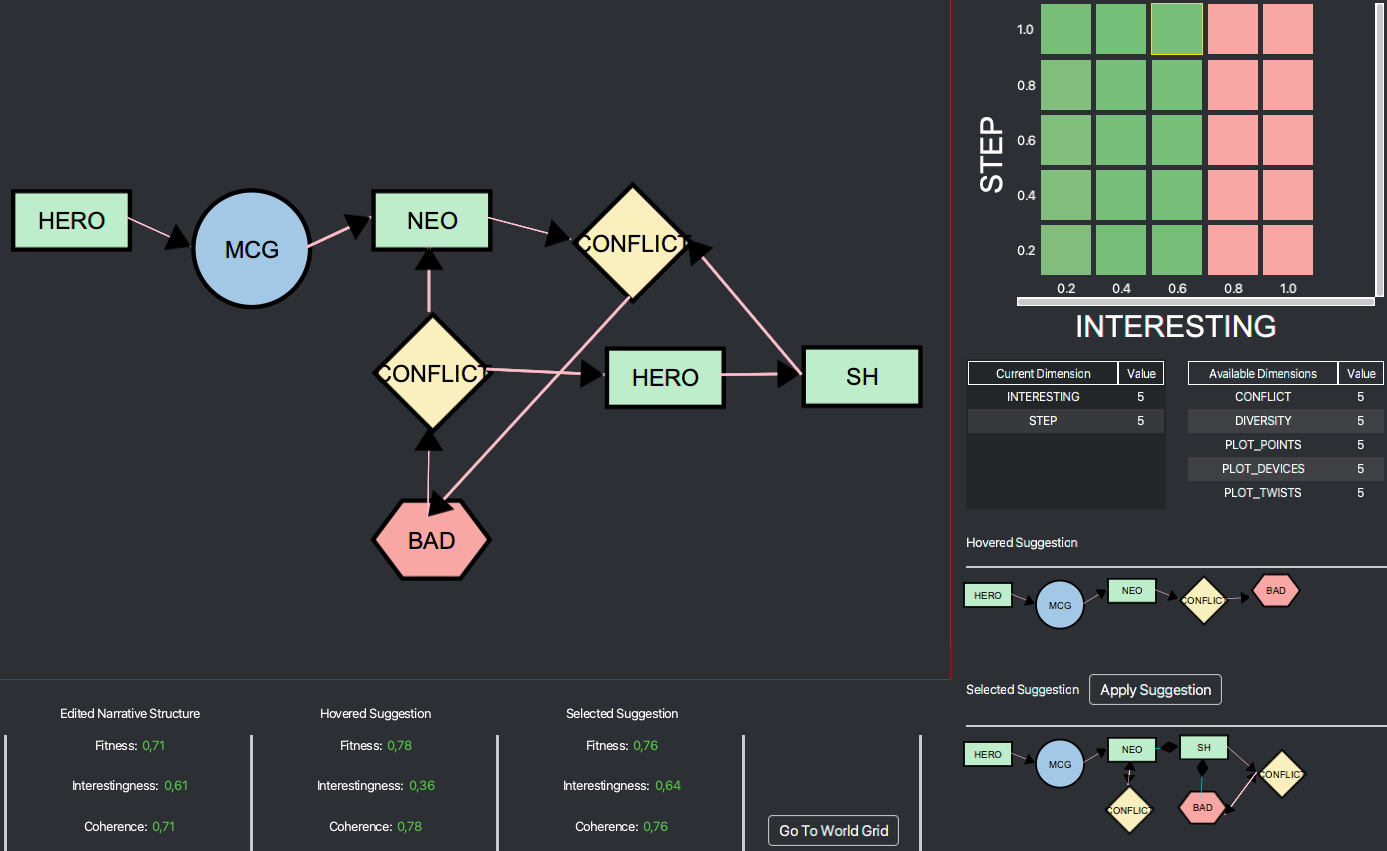
\includegraphics[width=\textwidth]{figures/current_GUI_fixed.png}
\caption{The Story Designer screen in the Evolutionary Dungeon Designer. In the center, there is the main narrative graph being edited by the designer. to the right, the suggestion grid using the Interactive Constrained MAP-Elites (IC MAP-Elites), the possible dimensions to be used, and two inspected suggestions. At the bottom, Story Designer presents some extra information regarding fitness, interestingness, and coherence, for the designer's convenience.}
    \label{fig:story-screen}
\end{figure*}